\section{Introduction}

Graphics processing units (GPUs) have been increasingly deployed in
general-purpose application domains due to their significant
improvements in performance and performance-per-watt.
As depicted in Figure~\ref{fig:perf_per_watt}, the performance-per-watt
of GPUs outperforms highly that of traditional multicore CPUs.
Albeit energy efficient, GPUs still consume non-trivial power during
operation.
Commodity system software for GPUs is unfortunately not well designed to
control their power consumption while primarily tailored to accelerate
computations.
To the best of our knowledge, commodity system software does not employ
even a basic scheme of voltage and frequency scaling for GPUs, though
most computational pieces of GPU-accelerated systems are offloaded on to
GPUs.
In order to develop truly energy-efficient GPU-accelerated systems, it
is essential to identify the trade-off in power and performance 
of GPUs and its causal relation with CPUs.

\begin{figure}[!t]
\centering
 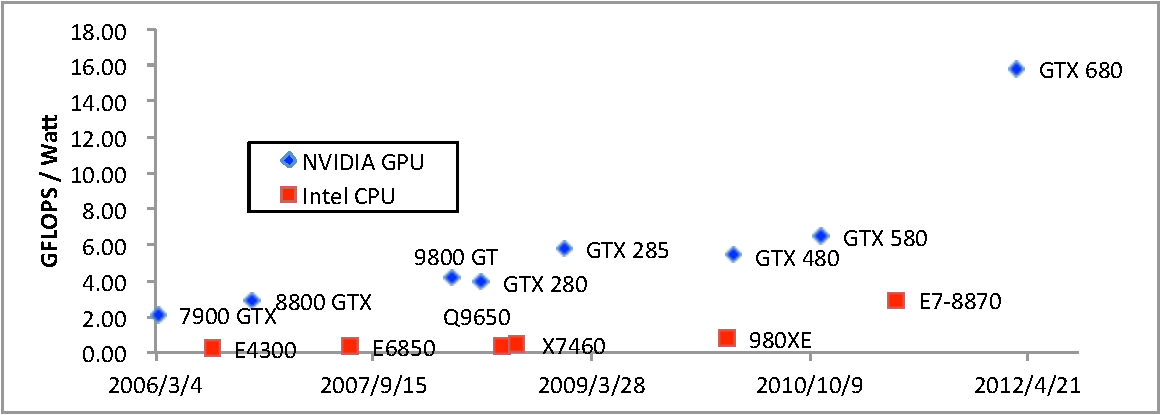
\includegraphics[width=0.46\textwidth]{figures/perf_per_watt.pdf}
 \label{fig:perf_per_watt}
 \caption{Performance-per-watt trends on representative NVIDIA GPUs and
 Intel CPUs.}
\end{figure}

Despite a rapid growth of GPU technology, there has been not much
understanding of power and performance implications of GPU-accelerated
systems.
According to vendor's specifications, the thermal design power (TDP) of
state-of-the-art GPUs is around 200W, while that of today's multicore
CPUs is typically below 100W.
Such a difference in the scale of TDP between CPUs and GPUs prevents
system designers from predicting the power and performance of
GPU-accelerated systems, which makes it difficult, if not impossible, to
optimize their energy savings.
Previous work~\cite{Hong2009,Hong2010,Jiao2010,Lee2011,Nagasaka2010} on
the power and performance analysis of GPU-accelerated systems are based
on either simulation studies or limited hardware functionality.
None of previous work has ever disclosed a fundamental approach to the
power and performance analysis of GPU-accelerated systems.

The contribution of this paper is to provide a power and performance
analysis of GPU-accelerated systems using NVIDIA's \textit{Fermi}
architectures.
Specifically, we identify when to scale the frequency and voltage of
GPUs and CPUs in order to minimize overall system energy.
Our analysis opens up important problems of dynamic voltage and
frequency scaling (DVFS) algorithms for growing GPU-accelerated
systems.
We also provide an open method and tool to scale voltage and frequency
of GPUs.
The black box feature of current GPU drivers and runtimes prevents
researchers from tackling correlative power and performance optimization
problems.
Sharing such a common method and tool with researchers
would further facilitate use of GPUs.

The rest of this paper is organized as follows.
%Section~\ref{sec:background} describes the background and motivation
%behind this work.
Section~\ref{sec:platform} presents our system platform.
Section~\ref{sec:evaluation} provides our evaluation.
Section~\ref{sec:related_work} discusses related work, and this paper
concludes in Section~\ref{sec:conclusion}.
